\input{template.tex}

\begin{document}

\makeheader

One day, Christian, the CEO of \textit{Super Arrangement Productions}, noticed that his company
was not running as he wanted. His employees complained about the lack of motivation.
Therefore, Christian decided to hire the motivation agency \textit{KcMinsey} to send their best
coaches in order to motivate the people again.

The coaches are taught to always work the same way. First, all coaches are sent to one boss to
motivate them, starting with Christian himself. Since they are insecure, they always work together,
which does not increase their power to motivate.
Then, they separate and motivate the employees below that boss. Since the coaches are a bit lazy,
they do not help their colleagues when they reached the lowest level of the hierarchy.

Sadly, motivating people is very exhausting. That means, that each person trying to motivate
an employee suffers in their motivational level equally to the demotivation level an employee
has. But after that, employees are as motivated as their coach was after the talk. Then,
they will even support their coaches and become coaches themselves.

Some people are not motivatable at all. Probably, because \textit{KcMinsesy}'s coaches
are too exhausted when they reach them. That would also mean not being able to motivate the
employees below that person anymore.

Christian wants to know the fewest number of coaches he needs and the number
of unmotivatable persons in order to do company stuff to them.

\definecolor{lightred}{RGB}{255,102,102}
\begin{figure}[h!]
  \centering

  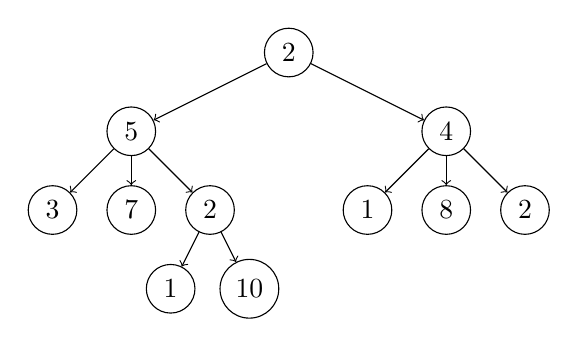
\begin{tikzpicture}[rn/.style={shape=circle,draw=black}]
    \node[rn] (1) at (3,4) {2};
    \node[rn] (2) at (1,3) {5};
    \node[rn] (3) at (0,2) {3};
    \node[rn] (4) at (1,2) {7};
    \node[rn] (5) at (2,2) {2};
    \node[rn] (6) at (1.5,1) {1};
    \node[rn] (7) at (2.5,1) {10};
    \node[rn] (8) at (5,3) {4};
    \node[rn] (9) at (4,2) {1};
    \node[rn] (10) at (5,2) {8};
    \node[rn] (11) at (6,2) {2};

    \path[->] (1) edge node {} (2);
    \path[->] (1) edge node {} (8);
    \path[->] (2) edge node {} (3);
    \path[->] (2) edge node {} (4);
    \path[->] (2) edge node {} (5);
    \path[->] (5) edge node {} (6);
    \path[->] (5) edge node {} (7);
    \path[->] (8) edge node {} (9);
    \path[->] (8) edge node {} (10);
    \path[->] (8) edge node {} (11);

  \end{tikzpicture}
  \caption{In Sample 1, all employees can be motivated.}
\end{figure}

\paragraph*{Input}

The input consists of three lines, describing a single test case.
The first line contains an integer $n$ ($1 \leq n \leq 10^5$), the number of employees and the motivational level $l$ of the coaches ($1 \leq l \leq 10^5$).
The second line contains $n$ integers. The $i$th integer is $m_i$ ($-10^6 \leq m_i \leq 10^6$), the motivational level of employee $i$.
The third line contains $n - 1$ integers. The $i$th integer is $b_{i+1}$ ($1 \leq b_{i+1} < i + 1$), the direct boss of colleague $i + 1$.

\paragraph*{Output}

Firstly, output the minimal number of coaches required to motivate the company.
Secondly, output the number of unmotivatable employees, followed by the numbers of those employees.


\begin{samples}
  \sample{sample1}
  \sample{sample2}
  \sample{sample3}
\end{samples}

\end{document}
